\documentclass{ds-report}

\usepackage[T1]{fontenc}
\usepackage{graphicx}
\usepackage{lmodern}
\usepackage{lscape}

\assignment{Java RMI} % Set to `Java RMI`, `Java EE` or `Google App Engine`.
\authorOne{Thomas Bamelis} % Name of first team partner.
\studentnumberOne{r0640219} % Student number of first team partner.
\authorTwo{Michiel Jonckheere} % Name of second team partner.
\studentnumberTwo{r0665594}  % Student number of second team partner.

\begin{document}
	\maketitle

	After the text answering the question, some clarifying pictures have been included.

	\paragraph{Question 1} 
	The client looks up information he needs for making a quote. When a client makes a quote with certain constraints, it asks for a quote to the car rental agency who returns the first available quote at one of the registered car companies. 
	The client can do this for a number of quotes, which are all saved to his session. When the client wants to confirm his quotes, he notifies the car rental agency. The car rental agency tries to confirm all quotes at the relevant car rental companies. If one fails, the already confirmed reservations are cancelled and the client is notified of the failure.\\
	
	On pages \pageref{startSession} - \pageref{reservationFails} are some sequence diagrams to illustrate it.
	
	
	\paragraph{Question 2}
	If an object of the class must be sent over the wire, the class must be serializable. This interface streams the object into a sequence of bytes and the receiver can restore the bytestream to the object. So each parameter or return value of remote methods must be serializable  (so also when it is contained in an object which has to be serializable). E.g. we had to make the class CarType serializable. 
	
	
	\paragraph{Question 3} 
	When a remote process wants to call a method on a local object. 
	
	\paragraph{Question 4}
	The data to be transmitted between client and server and back are the arguments and the return value of the remote call. In this case it has to be a string that contains the name of the client and the return will be an integer which contains the number of reservations of the specific renter.
	
	\paragraph{Question 5} 
	%First the client to CRA communication:\\
	The client and CRA (car rental agency) are on a different server. The client uses a CRA-stub which it looks up on a registry on the CRA-server to receive manager and reservation session-stubs. Interacting with the CRA is then done through this sessions. Every session on the client is a remote interface for a session object on the CRA-server. The session object then interacts locally with the CRA-object on the CRA-server. \\
	
	All interaction runs through the CRA-object and the client never directly talks to a CRC (car rental company). \\
	
	The CRA interacts with different CRC's which are all on their own remote servers. The CRA uses an interface to a remote CRC-object when interaction is necessary. The CRA keeps a list of interfaces of the registered CRC's. The only registry is located on the CRA and everybody interacts with it. When a CRC wants to register itself it pushes itself to this remote registry and notifies the CRA through a managersession. \\
	
	A diagram is added on page \pageref{designreport1} and \pageref{designreport2}.
	
	\paragraph{Question 6} 
	The CRA uses a hashmap with as key the name of the company and as value an interface stub to the remote object. A CRC pushes itself on to the registry before notifying the CRA with the name by which it can lookup the interface. The CRC is thus responsible for being available and staying available on the server while it is registered in the CRA.\\
	
	We chose this approach because of the ease of implementation and the lack of extra specification in the assignment.
	The first assignment also left this responsibility to the CRC.
	We realize this is not a viable solution in reality and leaves much room for error on the CRC side, but we prioritized our efforts on the running of the application and not on the bootstrap procedure.
	
	\paragraph{Question 7} 
	When a session is created it is created on the CRA-server and it pushes itself to registry. The CRA-server then sends the lookup name to the client for it to be used. When the client is done with the session, he calls close session on the remote interface to the remote object. The remote object then removes itself from the registry, thus removing the last local reference to it causing de garbage collector to collect the session. \\
	
	We chose this approach for a couple of reasons.
	The sessions are basically a facade pattern to their functionality. This is enforced by the session being a remote object.
	We also noticed this approach in java EE.
	It is more secure because no arbitrary calls can be made to the CRA and everything has to pass (= authenticate and authorize) through the beans.
	The functionality of the session was rather basic, but as beans get more complex (e.g. storing the list of quotes) and thus one session function call uses multiple calls to the CRA, this would greatly increase RMI overhead if the session would not be local to the CRA.
	
	\paragraph{Question 8} 
	Java RMI doesn't create copies of instances, so if an object is accessed by multiple clients, they all use the same object. That's why the objects that can be accessed by multiple threads must be made thread-safe.\\
	
	
	When a write is done, which is a change to a CRC-object, the CRA blocks any other call. So it's impossible for bad read to happen this way. Blocking is only necessary when quotes are being confirmed. We chose this approach because if the client can read incorrect information, he will e.g. be able to create invalid quotes. These will result in errors and the client will have to recall his methods to check which cartypes actually are available, which would be the same as waiting for the block to end.
	In general only read-read can be done safely at the same time, which is why we chose this approach.
	 
	
	\paragraph{Question 9} 
	The scalability is affected in that only one client can confirm at a time and while confirming no other clients can do anything. When there would be a lot of clients, this could be a potential bottleneck. 
	More scaleable approaches could have been possible such as only blocking car companies int the list of quotes, or blocking a car rental company only when a quote is being confirmed.
	These approaches would have been more complex to implement, increase the amount of rollbacks and also could introduce the problem of deadlocks.
	Because of time constraints and the lack of necessity we chose our more simple but less scalable solution.
	It is modeled after how distributed systems lock and would ask if everybody is able to commit (our ask and commit is done in one step though combined with a rollback) and only release after the process (confirmQuotes) using the resources (CRCs) terminates.
	
	\clearpage
	
	% You can include diagrams here.
	
	\begin{landscape}
		\begin{figure}
			\label{startSession}
			\centering
			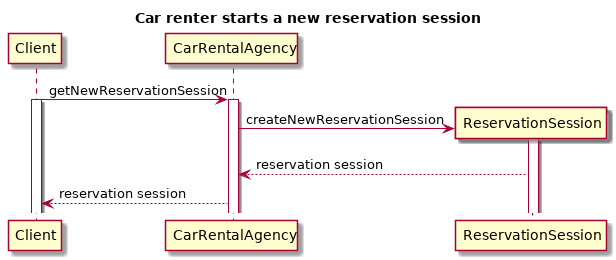
\includegraphics[width=\paperwidth]{../diagrams/sequenceDiagrams/startSession.png}
		\end{figure}
	\end{landscape}
	
\clearpage
	\begin{landscape}
		\begin{figure}
			\label{reserveCars}
			\centering
			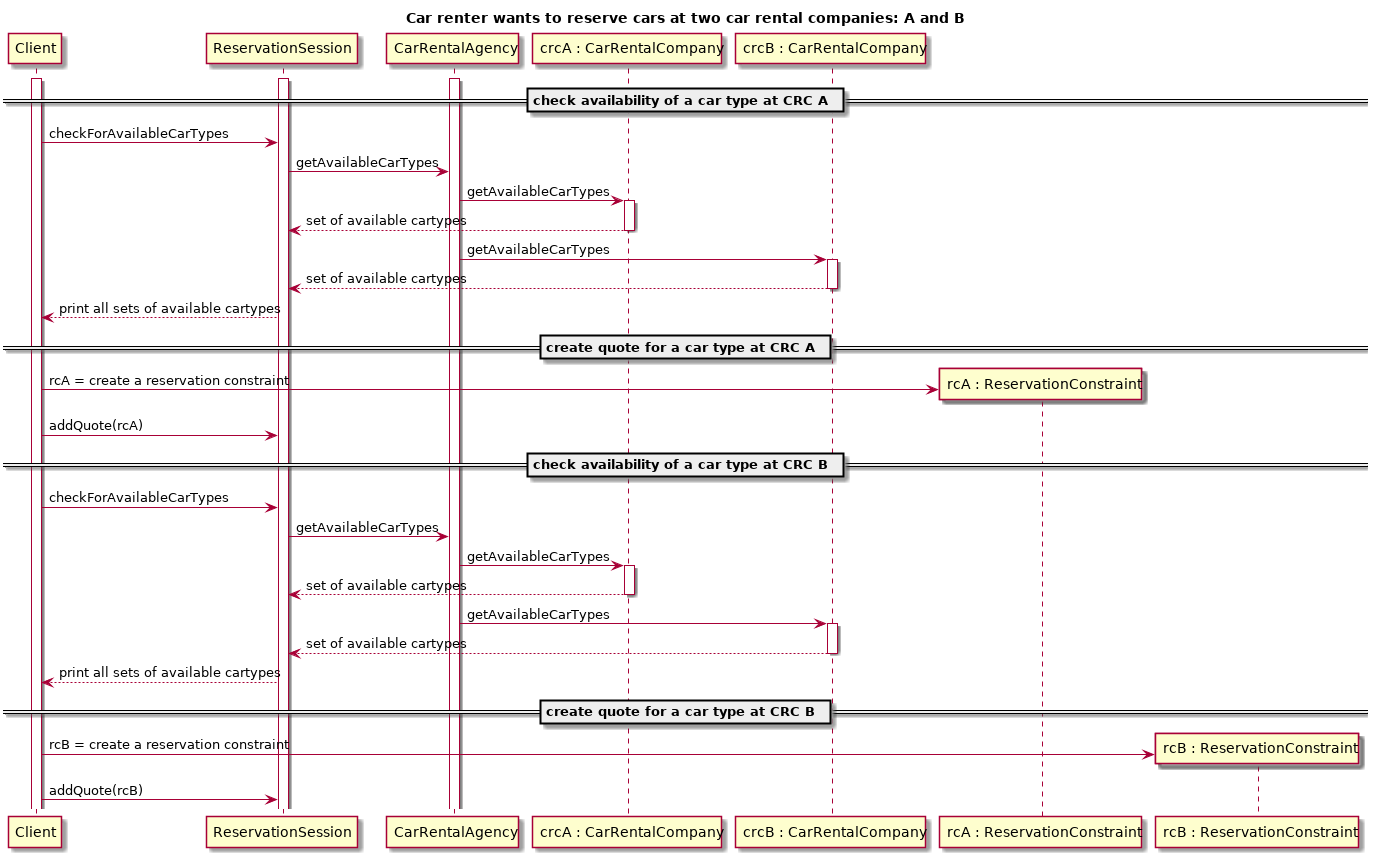
\includegraphics[width=\paperwidth]{../diagrams/sequenceDiagrams/reserveCars.png}
		\end{figure}
	\end{landscape}
	
\clearpage
	\begin{landscape}
		\begin{figure}
			\label{reservationSucceeds}
			\centering
			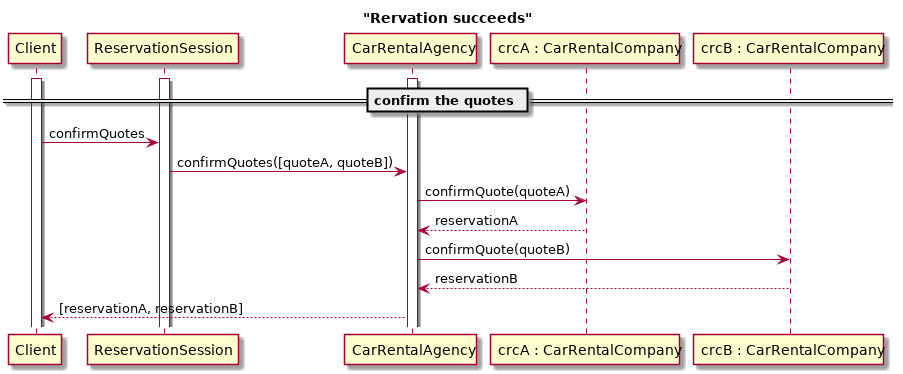
\includegraphics[width=\paperwidth]{../diagrams/sequenceDiagrams/reservationSucceeds.png}
		\end{figure}
	\end{landscape}
\clearpage
	\begin{landscape}
		\begin{figure}
			\label{reservationFails}
			\centering
			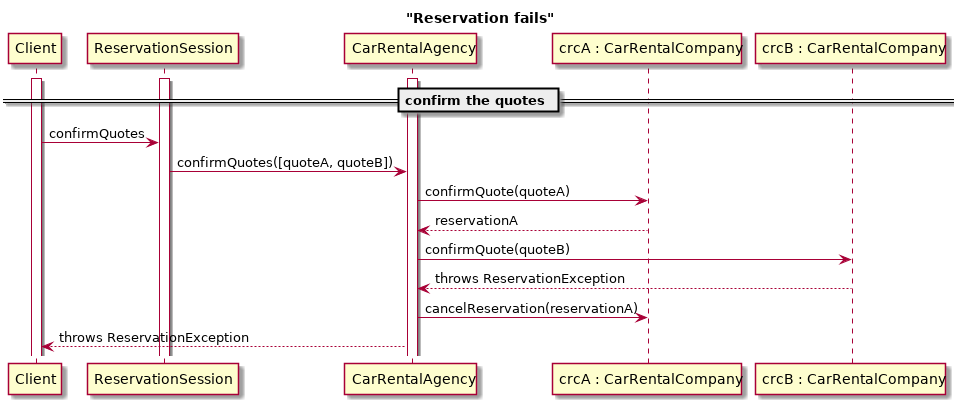
\includegraphics[width=\paperwidth]{../diagrams/sequenceDiagrams/reservationFails.png}
		\end{figure}
	\end{landscape}
\clearpage
\begin{landscape}
	\begin{figure}
				\label{designreport1}
		\centering
		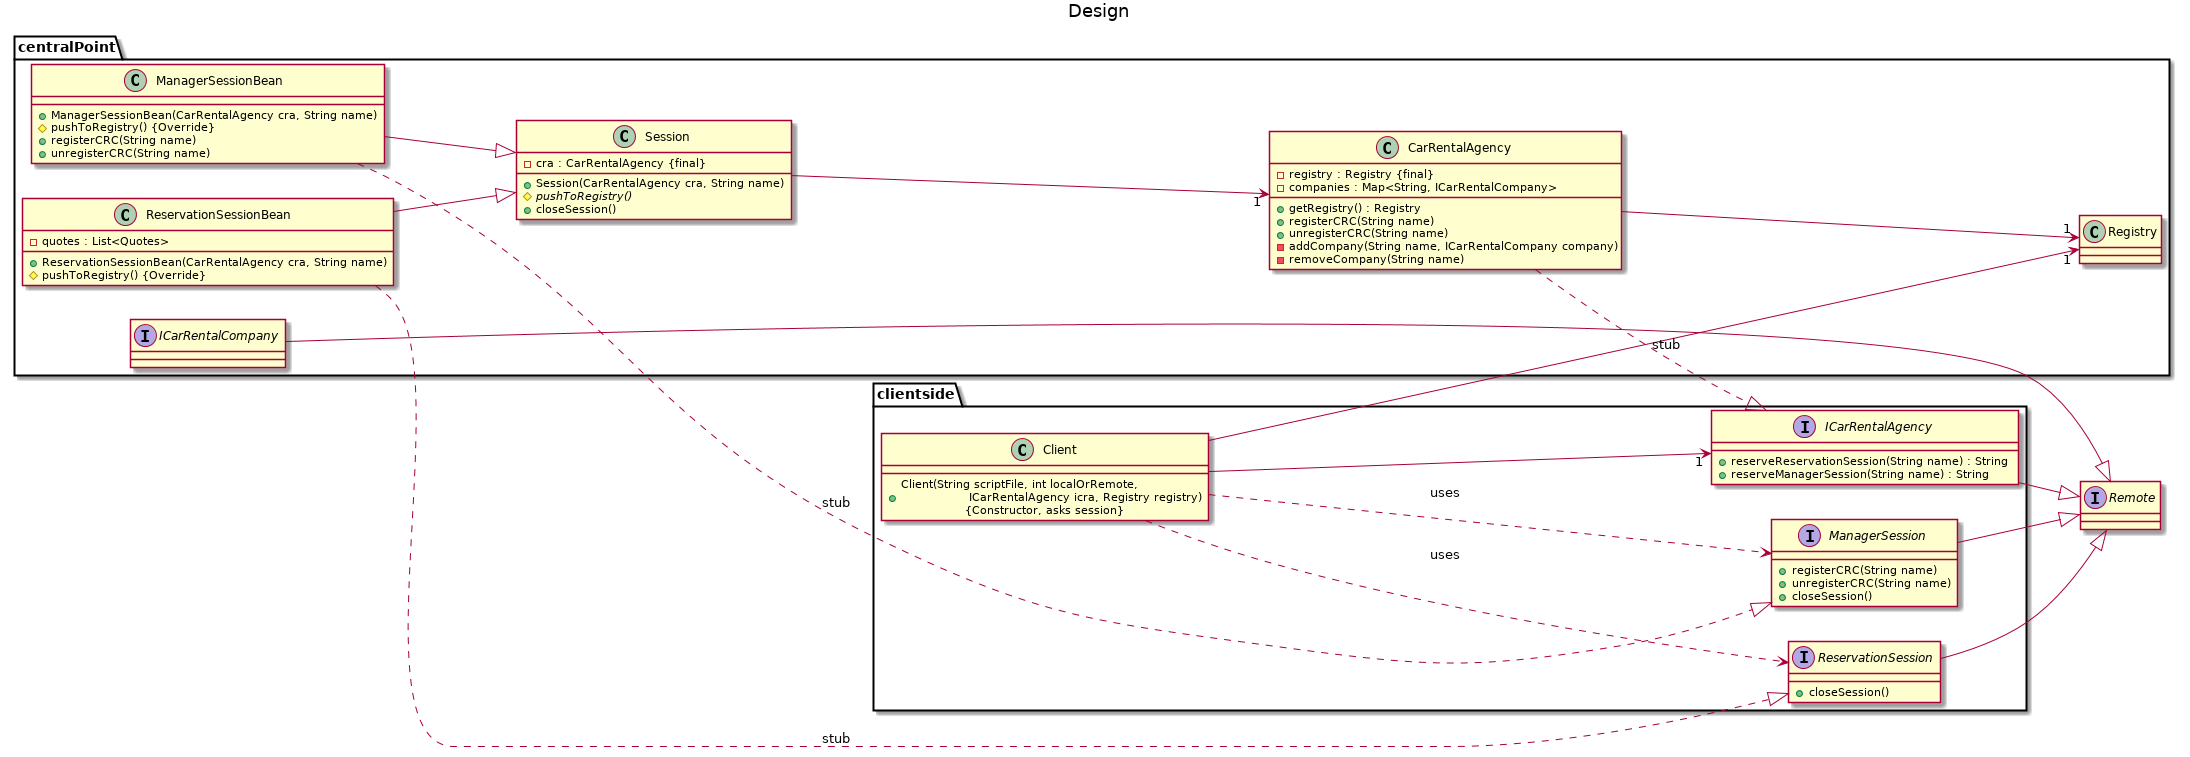
\includegraphics[width=\paperwidth]{../diagrams/design_report_1.png}
	\end{figure}
\end{landscape}
\clearpage
\begin{landscape}
	\begin{figure}
		\label{designreport2}
		\centering
		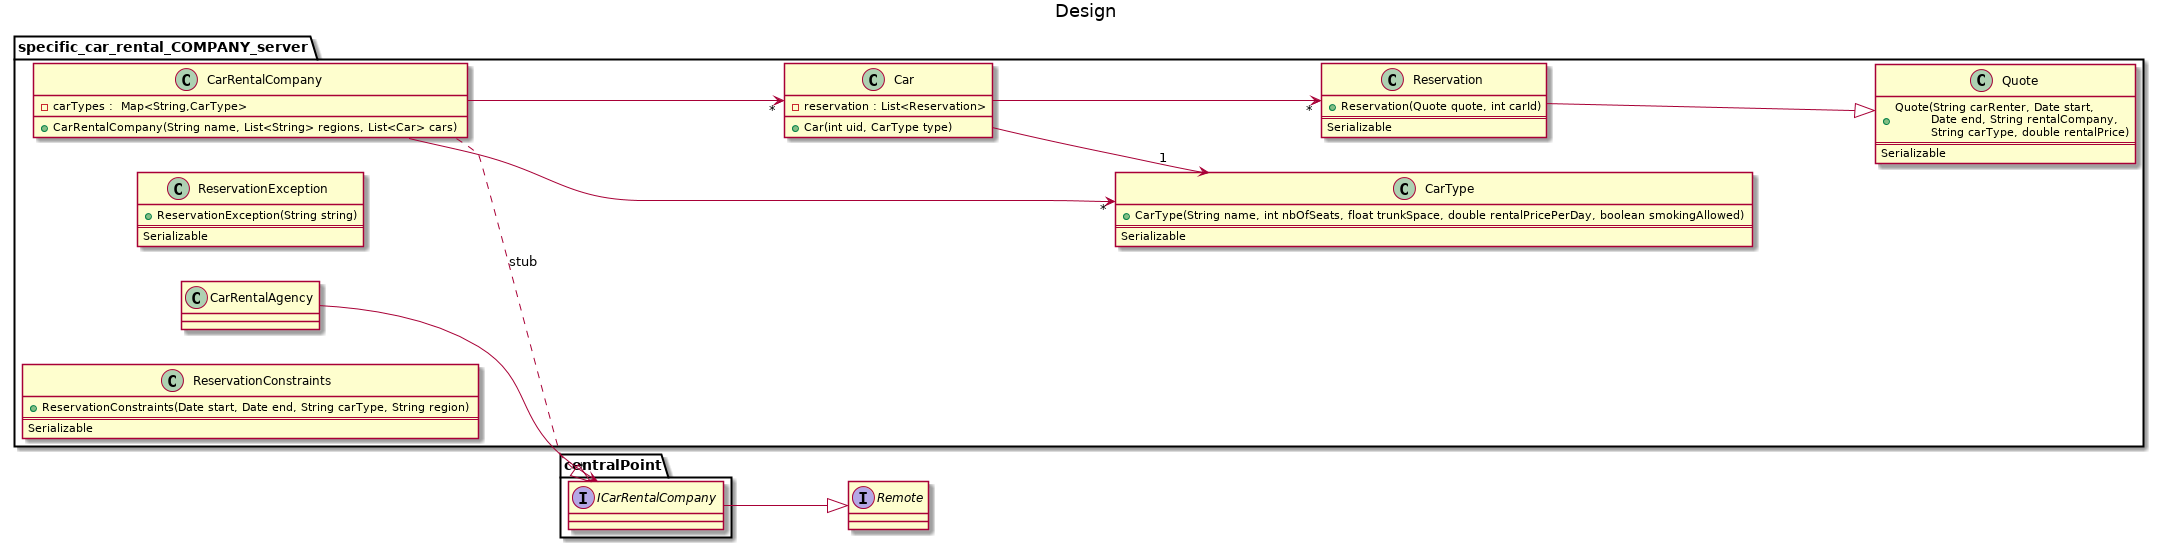
\includegraphics[width=\paperwidth]{../diagrams/design_report_2.png}
	\end{figure}
\end{landscape}

\end{document}
